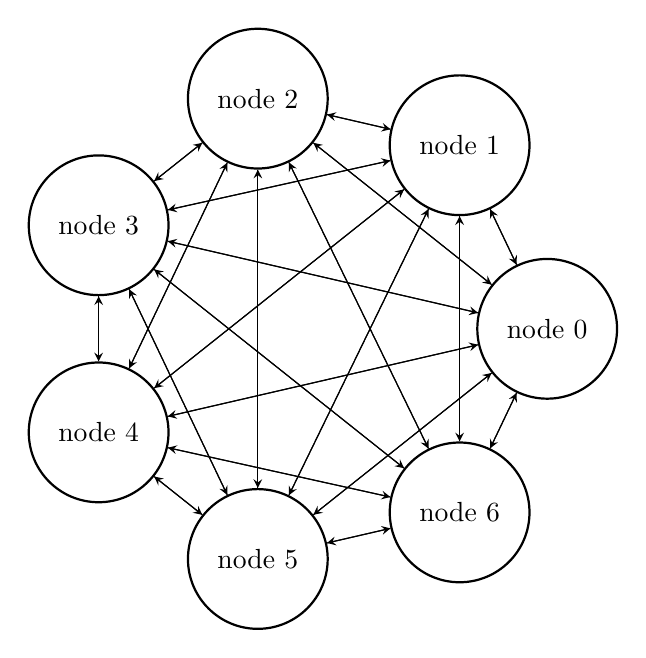
\begin{tikzpicture}[node distance=0.5cm,auto,>=stealth]
	\begin{scope}[baseline=(current bounding box.center)]
		\tikzstyle{knode}=[circle,draw=black,thick,inner sep=8pt,baseline=(current bounding box.center)]
		\node[knode] (n0) at (0:3cm) {node 0};
		\node[knode] (n1) at (51:3cm) {node 1};
		\node[knode] (n2) at (103:3cm) {node 2};
		\node[knode] (n3) at (154:3cm) {node 3};
		\node[knode] (n4) at (206:3cm) {node 4};
		\node[knode] (n5) at (257:3cm) {node 5};
		\node[knode] (n6) at (309:3cm) {node 6};
		%arrows
		\draw[->] (n0)--(n1);
		\draw[->] (n0)--(n2);
		\draw[->] (n0)--(n3);
		\draw[->] (n0)--(n4);
		\draw[->] (n0)--(n5);
		\draw[->] (n0)--(n6);
		\draw[->] (n1)--(n0);
		\draw[->] (n1)--(n2);
		\draw[->] (n1)--(n3);
		\draw[->] (n1)--(n4);
		\draw[->] (n1)--(n5);
		\draw[->] (n1)--(n6);
		\draw[->] (n2)--(n0);
		\draw[->] (n2)--(n1);
		\draw[->] (n2)--(n3);
		\draw[->] (n2)--(n4);
		\draw[->] (n2)--(n5);
		\draw[->] (n2)--(n6);
		\draw[->] (n3)--(n0);
		\draw[->] (n3)--(n1);
		\draw[->] (n3)--(n2);
		\draw[->] (n3)--(n4);
		\draw[->] (n3)--(n5);
		\draw[->] (n3)--(n6);
		\draw[->] (n4)--(n0);
		\draw[->] (n4)--(n1);
		\draw[->] (n4)--(n2);
		\draw[->] (n4)--(n3);
		\draw[->] (n4)--(n5);
		\draw[->] (n4)--(n6);
		\draw[->] (n5)--(n0);
		\draw[->] (n5)--(n1);
		\draw[->] (n5)--(n2);
		\draw[->] (n5)--(n3);
		\draw[->] (n5)--(n4);
		\draw[->] (n5)--(n6);
		\draw[->] (n6)--(n0);
		\draw[->] (n6)--(n1);
		\draw[->] (n6)--(n2);
		\draw[->] (n6)--(n3);
		\draw[->] (n6)--(n4);
		\draw[->] (n6)--(n5);
	\end{scope}
\end{tikzpicture}